% Template created by Robert Maier, 2013
\documentclass[t,plaincaption]{beamer}

\mode<presentation>
{
	\usepackage{theme_cvpr/beamerthemeCVPR}
	\setbeamercovered{transparent}
}

\usepackage{verbatim}

% Use xelatex to use TTF fonts 
\usepackage{fontspec}
\setsansfont{Arial}

% set the bibliography style
%\bibliographystyle{abbrv}
\bibliographystyle{apalike}

% set document information
\def\titleEn{Random GP Forest}
\def\authorName{Raphael Dümig, Andreas Wiedemann, Nan Liu, Dragomir Nikolic\\
\vspace{0.5cm}
Supervisor: Dr. habil. Rudolph Triebel}
\title[\titleEn]{\titleEn}
\author[Raphael Dümig, Andreas Wiedemann, Nan Liu, Dragomir Nikolic: \titleEn]{\authorName}
\date{July 27, 2015}


\begin{document}

\frame{
\titlepage 
}

\frame{
\frametitle{Outline}

\tableofcontents
}


\section{Problem}
\frame{
\frametitle{Problem}

\begin{columns}[t]
\begin{column}{0.45\linewidth}
\begin{itemize}
\item Gaussian Process (GP)
\begin{itemize}
\item high training time complexity	
\end{itemize}
\vspace{0.5cm}
\item Random Forest (RDF)
\begin{itemize}
\item 	moderate accuracy rate
\end{itemize}
%\vspace{0.5cm}
\end{itemize}
\end{column}

\begin{column}{0.65\linewidth}
\begin{figure}[t]
\centering

\begin{center}
\hspace{-3cm}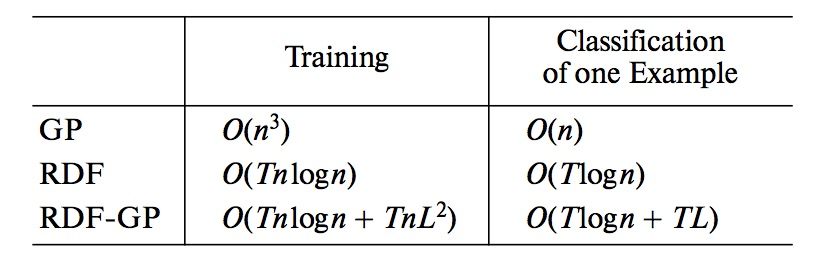
\includegraphics[width=3cm,height=1cm]{time}
\end{center}
\vspace{0.3cm}
\scriptsize{Table 1: Computational complexity: n denotes the number of training examples, L refers to the maximum number of examples a GP classifier is learned within a leaf, T is the number of decision trees in the forest$_{[1]}$.}

\end{figure}
\end{column}
\end{columns}
}


\section{Objective}
\frame{
\frametitle{Objective}

\begin{columns}[t]
\begin{column}{0.5\linewidth}
\begin{itemize}
\item Combining RDF and GP (RDF-GP)
\begin{itemize}
\item enable accurate classification in large-scale settings
\item GP: state-of-the-art recognition performance
\item RDF:  applied to large-scale dataset
\end{itemize}
\end{itemize}
\end{column}

\begin{column}{0.5\linewidth}
\begin{figure}[t]
\centering
\hspace{-2.5cm}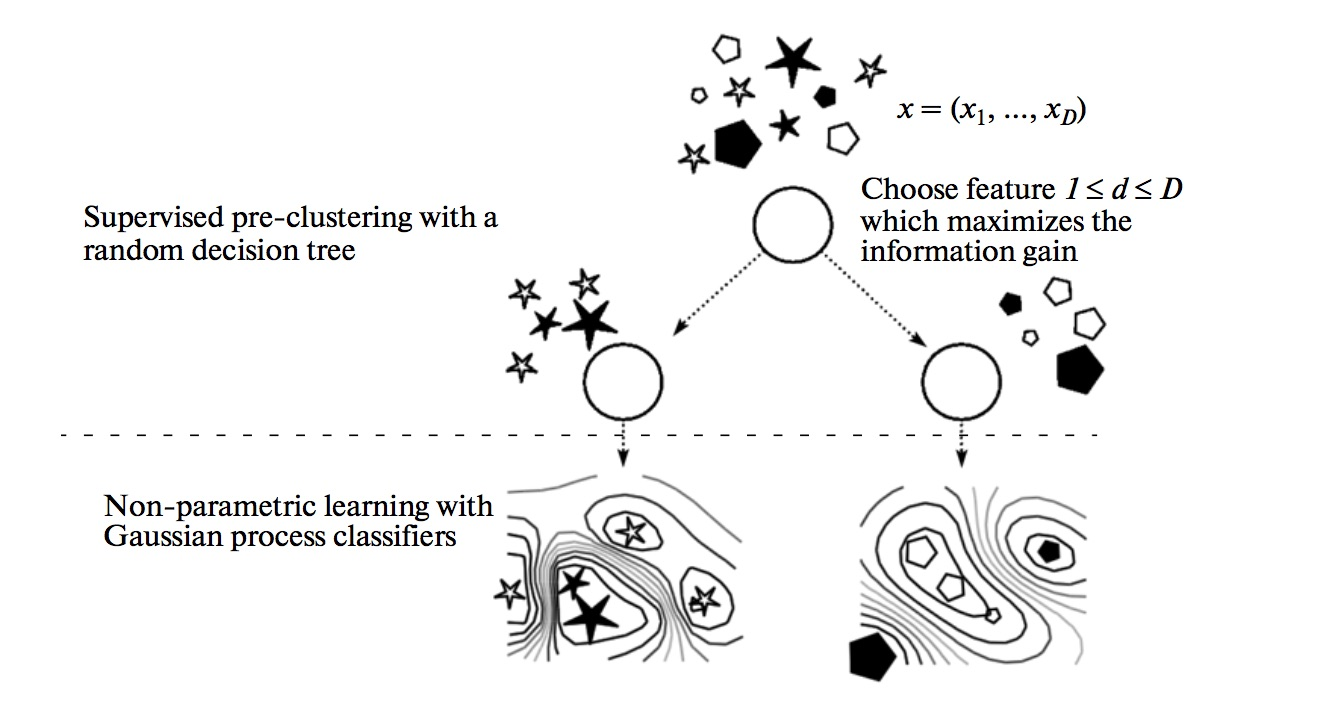
\includegraphics[width=0.5\linewidth]{fig1}

%\vspace{0.5cm}
\scriptsize{Figure 1: RDF is used to cluster the data in a supervised manner and a GP classifier is used to separate classes in each leaf$_{[1]}$.}
\label{fig1}
\end{figure}
\end{column}
\end{columns}
}


\section{Milestones}
\frame{
\frametitle{Milestones}

\begin{itemize}
\item Get GP classifier working \{3 weeks\}
\vspace{0.5cm}
\item Get online RDF working \{2 weeks\}
\vspace{0.5cm}
\item Combine GP and online RDF \{5 weeks\}
\end{itemize}
}

\section{Implementation}
\frame{
\frametitle{Implementation}

\begin{itemize}
\item language: C++
\item IDE : Ubantu ......
\end{itemize}

}

%\section{Implementation}
\frame{
\frametitle{Implementation}

\begin{itemize}
\item GP [Raphael Dragomir]
\begin{itemize}
\item library:
\item challenge:
\item solutions:
\end{itemize}
\end{itemize}

}

%\section{Implementation}
\frame{
\frametitle{Implementation}

\begin{columns}[t]
\begin{column}{0.5\linewidth}
\begin{itemize}
\item  RDF [Andreas Nan]
\begin{itemize}
\item OpenCV library, faild! 
\item Challenge: online version
\item Solution: Open source code from Amir Saffari et.al.[3]
\end{itemize}
\end{itemize}
\end{column}

\begin{column}{0.5\linewidth}
\begin{figure}[t]
\centering
\hspace{-2.8cm}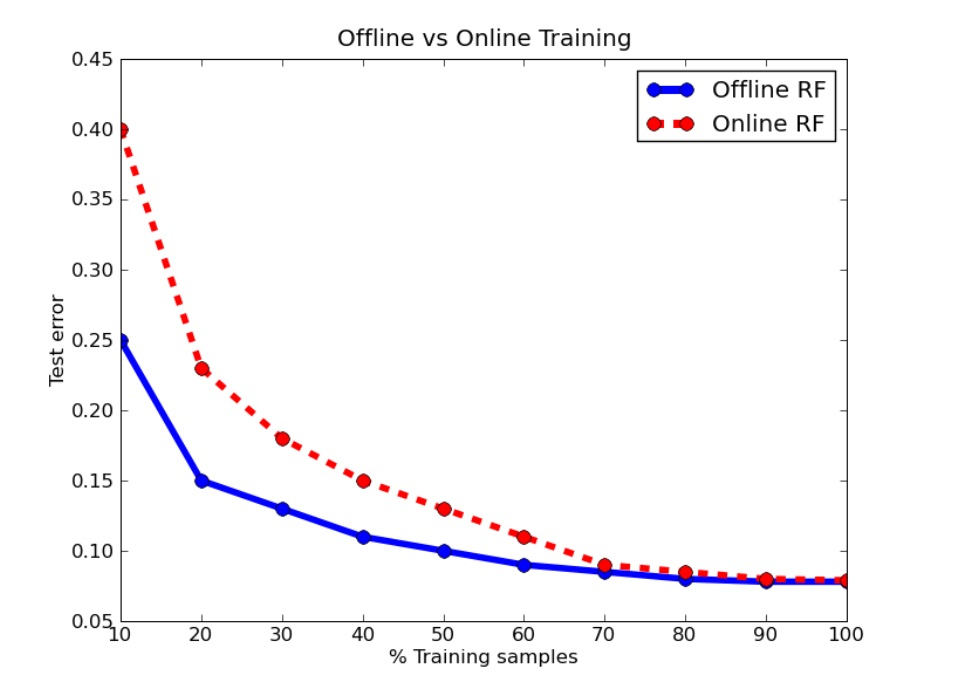
\includegraphics[width=3cm,height=1.5cm]{rdf_perf_onoff}

\scriptsize{Figure 2: Classification error with respect to the ratio of labeled samples for off-line and on-line training with increasing number of training samples$_{[3]}$.}
\label{fig2}
\end{figure}
\end{column}
\end{columns}
}

%\section{Implementation}
\frame{
\frametitle{Implementation}

\begin{itemize}
\item Combining GP with online RDF
\begin{itemize}
\item Challenge 1:  when to train GP?
\item Solution:  buffer
\item Challenge 2:  multiclassification?
\item Solution:  train n GPCs for each leaf node
\end{itemize}
\end{itemize}
}


%\section{Implementation}
\frame{
\frametitle{Implementation}

\begin{itemize}
\item What the system is capable of?
\begin{itemize}
\item GP classification
\item RDF classification
\item RDF-GP classification
\item binary and multi classification
\item online version
\end{itemize}
\end{itemize}
}

\section{Experiments and Evaluation}
\frame{
\frametitle{Experiments and Evaluation}
\begin{itemize}
\item Data: RGB-D Dataset$_{[2]}$ 
\end{itemize}

}

 
\section{Conclusion and Future Work}
\frame{
\frametitle{Conclusion and Future Work}

\begin{itemize}
\item Our Contributions:
\begin{itemize}
\item combined GP and RDF
\item implemented online version
\item obtained multi classifier
\end{itemize}
\end{itemize}

\begin{itemize}
\item Advantages:
\begin{itemize}
\item good accuracy maintained
\item substantially faster than the full GP classifier
\end{itemize}
\end{itemize}


\begin{itemize}
\item Future Work:
\begin{itemize}
\item parameter optimization 
\item using GPU for speed optimization
\end{itemize}
\end{itemize}

}

\frame[allowframebreaks]{
\frametitle{Bibliography}
	\tiny
	\bibliography{bibliography} 
\begin{thebibliography}{99}
\bibitem{1}
B. Fröhlich, E. Rodner, M. Kemmler, and J. DenzlerI,	 “Large-Scale Gaussian Process Classification Using Random Decision Forests, ” ISSN 1054-6618, Pattern Recognition and Image Analysis, 2012, Vol. 22, No. 1, pp. 113–120, 2012. 

\bibitem{2}
Kevin Lai, Liefeng Bo, Xiaofeng Ren, and Dieter Fox.  A Large-Scale Hierarchical Multi-View RGB-D Object Dataset. http://rgbd-dataset.cs.washington.edu

\bibitem{3}
Amir Saffari, Christian Leistner, Jakob Santner, Martin Godec, and Horst Bischof, "On-line Random Forests," 3rd IEEE ICCV Workshop on On-line Computer Vision, 2009.
\end{thebibliography}
}

\end{document}
